\runningheader{SAT Mathematics}{Drill Set 8}{Page \thepage\ of \numpages}

\begingradingrange{sat-drill-08}
\subsection*{SAT Drill 8}


\question[1]
The $x$-intercept of the graph shown is $(x, 0)$. What is the value of $x$?
\insertimage{0.40}{images/2025_06_15_5ccb8dd1752fe76599e7g-021}{reference attached}
\solutionorbox{1in}

\question[1]
Which of the following could be the equation of the graph shown in the $xy$-plane?
\insertimage{0.40}{images/2025_06_15_5ccb8dd1752fe76599e7g-022}{reference attached}
\begin{choices}
  \choice $y=-\frac{1}{10} x(x-4)(x+5)$
  \choice $y=-\frac{1}{10} x(x-4)(x+5)^{2}$
  \choice $y=-\frac{1}{10} x(x-5)(x+4)$
  \choice $y=-\frac{1}{10} x (x-5)^{2}(x+4)$
\end{choices}

\question[1]
$$f(x)=4 x^{2}+64 x+262$$\\
The function $g$ is defined by $g(x)=f(x+5)$. For what value of $x$ does $g(x)$ reach its minimum?
\begin{choices}
  \CorrectChoice -13
  \choice -8
  \choice -5
  \choice -3
\end{choices}

\question[1]
The graph of $y=f(x)$ is shown, where the function $f$ is defined by $f(x)=a x^{3}+b x^{2}+c x+d$ and $a, b, c$, and $d$ are constants. For how many values of $x$ does $f(x)=0$?
\insertimage{0.40}{images/2025_06_15_5ccb8dd1752fe76599e7g-024}{reference attached}
\begin{choices}
  \choice One
  \choice Two
  \choice Three
  \choice Four
\end{choices}

\question[1]
The table shown includes some values of $x$ and their corresponding values of $y$.
\begin{center}
  \begin{tabular}{|c|c|}
    \hline
    $x$ & $y$ \\
    \hline
    0 & 0 \\
    \hline
    1 & 1 \\
    \hline
    2 & 8 \\
    \hline
    3 & 27 \\
    \hline
  \end{tabular}
\end{center}
Which of the following graphs in the $xy$-plane could represent the relationship between $x$ and $y$?
\begin{center}
  \begin{tabular}{cccc}
    A. & B. & C. & D. \\
    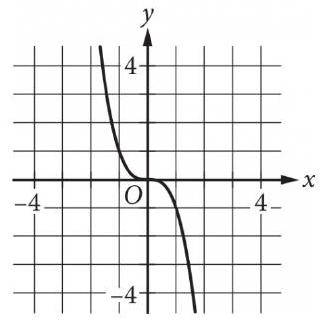
\includegraphics[width=0.23\textwidth]{images/2025_06_15_5ccb8dd1752fe76599e7g-025(2)} &
    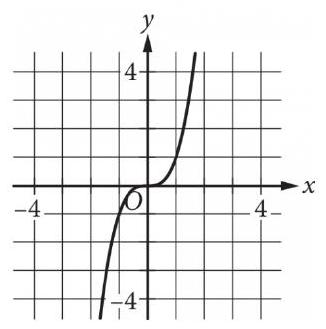
\includegraphics[width=0.23\textwidth]{images/2025_06_15_5ccb8dd1752fe76599e7g-025} &
    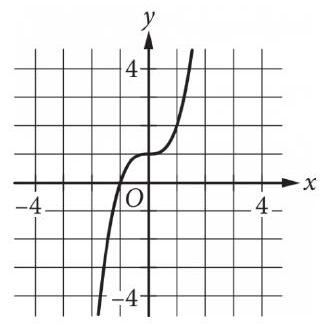
\includegraphics[width=0.23\textwidth]{images/2025_06_15_5ccb8dd1752fe76599e7g-025(3)} &
    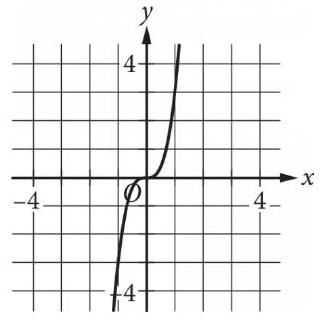
\includegraphics[width=0.23\textwidth]{images/2025_06_15_5ccb8dd1752fe76599e7g-025(1)} \\
  \end{tabular}
\end{center}
\begin{choices}
  \choice A
  \choice B
  \choice C
  \choice D
\end{choices}



















  
\question[1]
The function $f$ is defined by $f(x)=(x-6)(x-2)(x+6)$. In the $xy$-plane, the graph of $y=g(x)$ is the result of translating the graph of $y=f(x)$ up 4 units. What is the value of $g(0)$?
\begin{solution}
76
\end{solution}

\question[1]
A rectangle has a length of $x$ units and a width of $(x-15)$ units. If the rectangle has an area of 76 square units, what is the value of $x$?
\begin{choices}
  \choice 4
  \CorrectChoice 19
  \choice 23
  \choice 76
\end{choices}

\question[1]
A scientist initially measures 12,000 bacteria in a growth medium. 4 hours later, the scientist measures 24,000 bacteria. Assuming exponential growth, the formula $P=C(2)^{rt}$ gives the number of bacteria in the growth medium, where $r$ and $C$ are constants and $P$ is the number of bacteria $t$ hours after the initial measurement. What is the value of $r$?
\begin{choices}
  \choice $\frac{1}{12,000}$
  \CorrectChoice $\frac{1}{4}$
  \choice 4
  \choice 12,000
\end{choices}

\question[1]
A quadratic function models a projectile's height, in meters, above the ground in terms of the time, in seconds, after it was launched. The model estimates that the projectile was launched from an initial height of 7 meters above the ground and reached a maximum height of 51.1 meters above the ground 3 seconds after the launch. How many seconds after the launch does the model estimate that the projectile will return to a height of 7 meters?
\begin{choices}
  \choice 3
  \CorrectChoice 6
  \choice 7
  \choice 9
\end{choices}

\question[1]
The given equation relates the variables $x$ and $y$:
\[
  y=x^{2}-14x+22
\]
For what value of $x$ does the value of $y$ reach its minimum?
\begin{solution}
7
\end{solution}

\question[1]
Which expression is equivalent to $11x^{3}-5x^{3}$?
\begin{choices}
  \choice $16x^{3}$
  \CorrectChoice $6x^{3}$
  \choice $6x^{6}$
  \choice $16x^{6}$
\end{choices}

\question[1]
Which expression is equivalent to $50x^{2}+5x^{2}$?
\begin{choices}
  \choice $250x^{2}$
  \choice $10x^{2}$
  \choice $45x^{2}$
  \CorrectChoice $55x^{2}$
\end{choices}

\question[1]
The expression $(3x-23)(19x+6)$ is equivalent to the expression $ax^{2}+bx+c$, where $a$, $b$, and $c$ are constants. What is the value of $b$?
\begin{solution}
-419
\end{solution}

\question[1]
Which expression is equivalent to $20w-(4w+3w)$?
\begin{choices}
  \choice $10w$
  \CorrectChoice $13w$
  \choice $19w$
  \choice $21w$
\end{choices}


  




















\question[1]
Which expression is equivalent to $\frac{4}{4x-5}-\frac{1}{x+1}$?
\begin{choices}
  \choice $\frac{1}{(x+1)(4x-5)}$
  \choice $\frac{3}{3x-6}$
  \choice $-\frac{1}{(x+1)(4x-5)}$
  \CorrectChoice $\frac{9}{(x+1)(4x-5)}$
\end{choices}

\question[1]
Which of the following is equivalent to $3(x+5)-6$?
\begin{choices}
  \choice $3x-3$
  \choice $3x-1$
  \CorrectChoice $3x+9$
  \choice $15x-6$
\end{choices}

\question[1]
In the expression $$\frac{x^{2}-c}{x-b}$$, $b$ and $c$ are positive integers. If the expression is equivalent to $x+b$ and $x \neq b$, which of the following could be the value of $c$?
\begin{choices}
  \CorrectChoice 4
  \choice 6
  \choice 8
  \choice 10
\end{choices}

\question[1]
Which of the following expressions is equivalent to $\sqrt[3]{x^3y^6}$?
\begin{choices}
  \choice $y^{2}$
  \CorrectChoice $xy^{2}$
  \choice $y^{3}$
  \choice $xy^{3}$
\end{choices}

\question[1]
Which expression is equivalent to $(d-6)(8d^{2}-3)$?
\begin{choices}
  \choice $8d^{3}-14d^{2}-3d+18$
  \choice $8d^{3}-17d^{2}+48$
  \CorrectChoice $8d^{3}-48d^{2}-3d+18$
  \choice $8d^{3}-51d^{2}+48$
\end{choices}

\question[1]
If $x^{2}=a+b$ and $y^{2}=a+c$, which of the following is equal to $(x^{2}-y^{2})^{2}$?
\begin{choices}
  \choice $a^{2}-2ac+c^{2}$
  \CorrectChoice $b^{2}-2bc+c^{2}$
  \choice $4a^{2}-4abc+c^{2}$
  \choice $4a^{2}-2abc+b^{2}c^{2}$
\end{choices}

\question[1]
If the ordered pair $(x,y)$ satisfies the system of equations
\[
  \begin{aligned}
    & y=x^{2}-4x+4 \\
    & y=4-x
  \end{aligned}
\]
what is one possible value of $x$?
\begin{solution}
3
\end{solution}

\question[1]
An oceanographer uses the equation $$s=\frac{3}{2}p$$ to model the speed $s$, in knots, of an ocean wave, where $p$ represents the period of the wave, in seconds. Which of the following represents the period of the wave in terms of the speed of the wave?
\begin{choices}
  \CorrectChoice $p=\frac{2}{3}s$
  \choice $p=\frac{3}{2}s$
  \choice $p=\frac{2}{3}+s$
  \choice $p=\frac{3}{2}+s$
\end{choices}

























\question[1]
Which of the following is a solution to the equation $2x^{2}-4=x^{2}$?
\begin{choices}
  \choice 1
  \CorrectChoice 2
  \choice 3
  \choice 4
\end{choices}

\question[1]
The given equation relates the positive numbers $q$, $r$, and $s$:
\[
  q-29r=s
\]
Which equation correctly expresses $q$ in terms of $r$ and $s$?
\begin{choices}
  \choice $q=s-29r$
  \CorrectChoice $q=s+29r$
  \choice $q=29rs$
  \choice $q=-\frac{s}{29r}$
\end{choices}

\question[1]
In the given equation, $a$ and $b$ are positive constants:
\[
  57x^{2}+(57b+a)x+ab=0
\]
The product of the solutions to the given equation is $kab$, where $k$ is a constant. What is the value of $k$?
\begin{choices}
  \CorrectChoice $\frac{1}{57}$
  \choice $\frac{1}{19}$
  \choice 1
  \choice 57
\end{choices}

\question[1]
In the given equation, $b$ is a positive integer:
\[
  -x^{2}+bx-676=0
\]
The equation has no real solution. What is the greatest possible value of $b$?
\begin{solution}
51
\end{solution}

\question[1]
The given equation relates the distinct positive numbers $p$, $k$, and $j$:
\[
  p=\frac{k}{4j+9}
\]
Which equation correctly expresses $4j+9$ in terms of $p$ and $k$?
\begin{choices}
  \CorrectChoice $4j+9=\frac{k}{p}$
  \choice $4j+9=kp$
  \choice $4j+9=k-p$
  \choice $4j+9=\frac{p}{k}$
\end{choices}

\question[1]
If $3x^{2}-18x-15=0$, what is the value of $x^{2}-6x$?
\begin{solution}
5
\end{solution}

\question[1]
In the $xy$-plane, what is the $y$-coordinate of the point of intersection of the graphs of $y=(x-1)^{2}$ and $y=2x-3$?
\begin{solution}
1
\end{solution}

\question[1]
In the equation $2x^{2}-4x=t$, $t$ is a constant. If the equation has no real solutions, which of the following could be the value of $t$?
\begin{choices}
  \CorrectChoice -3
  \choice -1
  \choice 1
  \choice 3
\end{choices}

